\documentclass{beamer}

\usepackage[orientation=landscape,size=a0,scale=1.4,debug]{beamerposter}
\mode<presentation>{\usetheme{mlr}}

\usepackage[utf8]{inputenc} % UTF-8
\usepackage[english]{babel} % Language
\usepackage{hyperref} % Hyperlinks
\usepackage{ragged2e} % Text position
\usepackage[export]{adjustbox} % Image position
\usepackage[most]{tcolorbox}
\usepackage{listings} % for R code
\lstset{language=R,
    basicstyle=\small\ttfamily,
    stringstyle=\color{DarkGreen},
    otherkeywords={0,1,2,3,4,5,6,7,8,9},
    morekeywords={TRUE,FALSE},
    deletekeywords={data,frame,length,as,character},
    keywordstyle=\color{blue},
    commentstyle=\color{DarkGreen},
}

\title{mlr3tuning :\,: CHEAT SHEET} % Package title in header, \, adds thin space between ::
\newcommand{\packagedescription}{ % Package description in header
	The \textbf{mlr3tuning} package provides hyperparameter tuning for mlr3.
}

\newlength{\columnheight} % Adjust depending on header height
\setlength{\columnheight}{84cm} 

\newtcolorbox{codebox}{%
	sharp corners,
	leftrule=0pt,
	rightrule=0pt,
	toprule=0pt,
	bottomrule=0pt,
	hbox}

\newtcolorbox{codeboxmultiline}[1][]{%
	sharp corners,
	leftrule=0pt,
	rightrule=0pt,
	toprule=0pt,
	bottomrule=0pt,
	#1}

\newtcolorbox{codeboxinline}{%
	sharp corners,
	leftrule=0pt,
	rightrule=0pt,
	toprule=0pt,
	bottomrule=0pt,
	hbox,
	nobeforeafter,
	tcbox raise base}

\newcommand{\codeinline}[1]{\begin{codeboxinline}#1\end{codeboxinline}}

\begin{document}
\begin{frame}[fragile]{}
	\begin{columns}
		\begin{column}{.245\textwidth}
			\begin{beamercolorbox}[center]{postercolumn}
				\begin{minipage}{.98\textwidth}
					\parbox[t][\columnheight]{\textwidth}{
						\begin{myblock}{Intro}
							The mlr3tuning package is an extension for the \href{https://github.com/mlr-org/mlr3}{mlr3} package and provides R6 classes for hyperparameter tuning.
							\\
							\\
							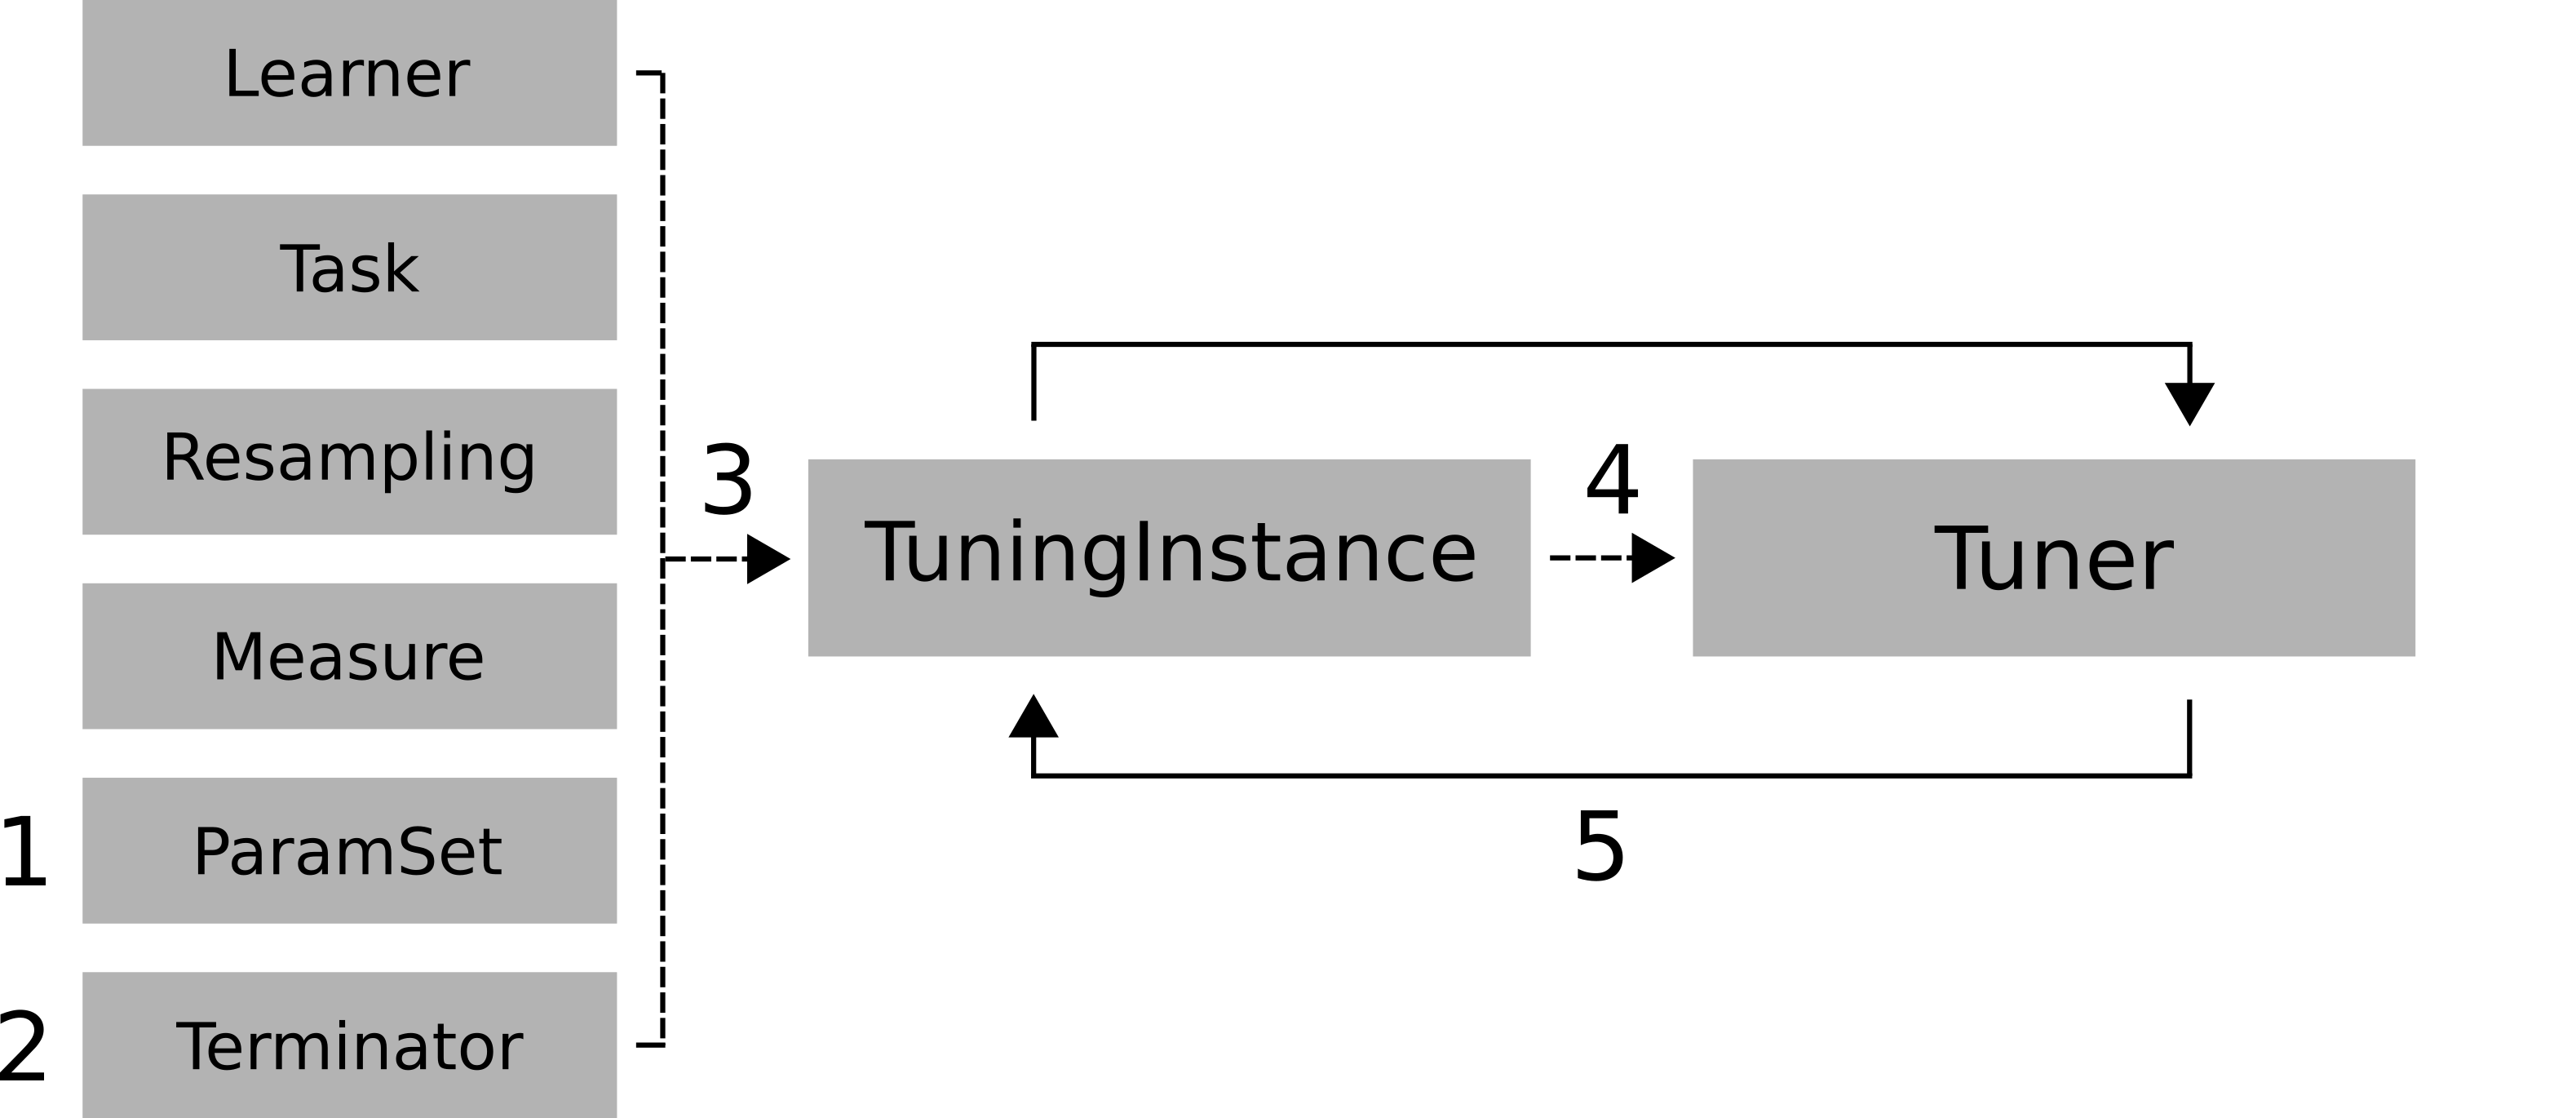
\includegraphics[width=\textwidth]{img/tuning_objects.png}
						\end{myblock}
						\begin{myblock}{ParamterSet}
						The \codeinline{ParamSet} defines the hyperparameter to tune and the tuning space.
						\\
						\begin{codeboxmultiline}[width=19cm]
							tune\_ps = \textbf{ParamSet}\$new(list(\\
							\hspace*{1ex}\textbf{ParamInt}\$new(id, lower, upper)\\
							\hspace*{1ex}\textbf{ParamDbl}\$new(id, lower, upper)))
						\end{codeboxmultiline}
						The \textit{id} refers to the hyperparameter of the learner. The \textit{lower} and \textit{upper} parameter define the bounds of the tuning space. 	
					\end{myblock}	
					\vfill}
				\end{minipage}
			\end{beamercolorbox}
		\end{column}
		\begin{column}{.245\textwidth}
			\begin{beamercolorbox}[center]{postercolumn}
				\begin{minipage}{.98\textwidth}
					\parbox[t][\columnheight]{\textwidth}{
						\begin{myblock}{Terminator}
						The Terminator determines when to stop the tuning. The package provides four Terminator classes:
						\\
						\begin{codebox}
							terminator = \textbf{TerminatorClockTime}\$new()
						\end{codebox}
						Terminate after a given time.
						\\
						\begin{codebox}
							terminator = \textbf{TerminatorEvals}\$new()
						\end{codebox}
						Terminate after a given amount of iterations. 
						\\
						\begin{codebox}
							terminator = \textbf{TerminatorPerfReached}\$new()
						\end{codebox}
						Terminate after a specific performance is reached.  
						\\
						\begin{codebox}
							terminator = \textbf{TerminatorStagnation}\$new()
						\end{codebox}
						Terminate when tuning does not improve.
						\\
						\begin{codebox}
							terminator = \textbf{TerminatorCombo}\$new()
						\end{codebox}
						A combination of the above in an ALL or ANY fashion.
						\\
						\begin{codebox}
							terminator = \textbf{term}(key, ...)
						\end{codebox}
						Get terminator by \textit{key} and construct terminator with settings (...) in one go. 
					\end{myblock}	
				\begin{myblock}{TuningInstance}
					The TuningInstance specifies a general search scenario. It evaluates the hyperparameter configurations proposed by the \codeinline{Tuner} and stores the results (s. Triggering the tuning).
					\\
					\begin{codeboxmultiline}[width=18cm]
						instance = \textbf{TuningInstance}\$new(\\
						\hspace*{1ex}task,\\
						\hspace*{1ex}learner,\\
						\hspace*{1ex}resampling,\\
						\hspace*{1ex}tune\_ps,\\
						\hspace*{1ex}terminator)
					\end{codeboxmultiline}
					The TuningInstance is constructed by supplying \textit{task}, \textit{learner}, \textit{resampling}, \textit{tune\_ps} and \textit{terminator}. 
					\\
				\end{myblock}	
					\vfill}
				\end{minipage}
			\end{beamercolorbox}
		\end{column}
		\begin{column}{.245\textwidth}
			\begin{beamercolorbox}[center]{postercolumn}
				\begin{minipage}{.98\textwidth}
					\parbox[t][\columnheight]{\textwidth}{
						\begin{myblock}{Tuner}
							The Tuner describes the tuning strategy. The package provides three algorithms:
							\\
							\begin{codebox}
								tuner = \textbf{TunerGridSearch}\$new()
							\end{codebox}
							Grid search.
							\\
							\begin{codebox}
								tuner = \textbf{TunerRandomSearch}\$new()
							\end{codebox}
							Random Search.
							\\
							\begin{codebox}
								tuner = \textbf{TunerGenSA}\$new()
							\end{codebox}
							Generalized Simulated Annealing.
							\\
							\begin{codebox}
								tuner = \textbf{trn}(key, ...)
							\end{codebox}
							Get tuner by \textit{key} and construct tuner with settings (...) in one go.
						\end{myblock}
						\begin{myblock}{Triggering the tuning}
							To start the tuning, the \codeinline{TuningInstance} is passed to the \codeinline{tune} method of the \codeinline{Tuner}.
							\\
							\begin{codebox}
								tuner\$\textbf{tune}(instance)
							\end{codebox}
							Starts the tuning.
							\\
							\begin{codebox}
								instance\$\textbf{archive}(unnest)
							\end{codebox}
							Returns all resampling results together with the used hyperparameters.
							\\
							\begin{codebox}
								instance\$\textbf{result}
							\end{codebox}
							Returns a list with the optimal hyperparameter configuration and the estimated performance.
						\end{myblock}
					\vfill}
				\end{minipage}
			\end{beamercolorbox}
		\end{column}
		\begin{column}{.245\textwidth}
			\begin{beamercolorbox}[center]{postercolumn}
				\begin{minipage}{.98\textwidth}
					\parbox[t][\columnheight]{\textwidth}{
						\begin{myblock}{Automatic Tuning}
						The \codeinline{AutoTuner} wraps a learner and augments it with an automatic tuning for a given set of hyperparameters. 
						\\
						\begin{codeboxmultiline}[width=18cm]
							at = \textbf{AutoTuner}\$new(
\\
							\hspace*{1ex}learner,
\\
							\hspace*{1ex}resampling,
\\
							\hspace*{1ex}measures,
\\
							\hspace*{1ex}tune\_ps,
\\
							\hspace*{1ex}terminator,
\\
							\hspace*{1ex}tuner)
						\end{codeboxmultiline}
						The \codeinline{AutoTuner} is constructed by supplying \textit{learner}, \textit{task},  \textit{resampling}, \textit{measures}, \textit{tune\_ps}, \textit{terminator} and \textit{tuner}. 
						\\
						\\
						The \codeinline{AutoTuner} inherits from the \codeinline{Learner} class and therefore can be used like any other learner.
						\\
						\begin{codebox}
							at\$\textbf{predict}(task, row\_ids)
						\end{codebox}
						Use the tuned \codeinline{Learner} in \codeinline{AutoTuner} to create a new \codeinline{Prediction} by suppling a \textit{task} and \textit{row\_ids}.
						\\
						\begin{codebox}
							at\$\textbf{train}(task)
						\end{codebox}
						Train the tuned \codeinline{Learner} in \codeinline{AutoTuner} on a new \textit{task}.
						\end{myblock}
					\vfill}
				\end{minipage}
			\end{beamercolorbox}
		\end{column}
	\end{columns}
\end{frame}
\end{document}
